% Created 2020-04-27 Mon 19:33
% Intended LaTeX compiler: pdflatex
\documentclass[11pt]{article}
\usepackage[utf8]{inputenc}
\usepackage[T1]{fontenc}
\usepackage{graphicx}
\usepackage{grffile}
\usepackage{longtable}
\usepackage{wrapfig}
\usepackage{rotating}
\usepackage[normalem]{ulem}
\usepackage{amsmath}
\usepackage{textcomp}
\usepackage{amssymb}
\usepackage{capt-of}
\usepackage{hyperref}
\usepackage{minted}
\usepackage{/home/ryan/Dropbox/profiles/Templates/LaTeX/ScreenStyle}
\usepackage[citestyle=numeric, bibstyle=numeric,hyperref=true,backref=true, maxcitenames=3,url=true,backend=biber,natbib=true]{biblatex}
\addbibresource{/home/ryan/Dropbox/Studies/Papers/references.bib}
%%% TeX-command-extra-options: "-shell-escape"
\author{Ryan Greenup}
\date{\today}
\title{}
\hypersetup{
 pdfauthor={Ryan Greenup},
 pdftitle={},
 pdfkeywords={},
 pdfsubject={},
 pdfcreator={Emacs 27.0.91 (Org mode 9.4)}, 
 pdflang={English}}
\begin{document}

\tableofcontents


\section{8.1 Analysing the Relationship Between Friends and Followers for Twitter Users}
\label{sec:org8d31234}
\subsection{8.1.1 Retrieve the posts from Twitter}
\label{sec:orgb56dc09}
relevant posts can be retrieved from twitter by utilising the \texttt{rtweet} package, packages can be loaded for use in \textbf{\textbf{\uline{R}}} thusly:

\begin{listing}[htbp]
\begin{minted}[]{r}
# Load Packages -----------------------------------------------------------
setwd("~/Dropbox/Notes/DataSci/Social_Web_Analytics/SWA-Project/scripts/")

if (require("pacman")) {
  library(pacman)
} else{
  install.packages("pacman")
  library(pacman)
}

pacman::p_load(xts, sp, gstat, ggplot2, rmarkdown, reshape2,
               ggmap, parallel, dplyr, plotly, tidyverse,
               reticulate, UsingR, Rmpfr, swirl, corrplot,
               gridExtra, mise, latex2exp, tree, rpart,
               lattice, coin, primes, epitools, maps, clipr,
               ggmap, twitteR, ROAuth, tm, rtweet, base64enc,
               httpuv, SnowballC, RColorBrewer, wordcloud,
               ggwordcloud, tidyverse, boot)
\end{minted}
\caption{\label{org6d215bf}Load the Packages for \textbf{\textbf{\emph{R}}}}
\end{listing}


The \texttt{rtweet} API will search for tweets that contain all the words of a query
regardless of uppercase or lowercase usage \cite{kearney2019}.

In order to leverage the \emph{Twitter} API it is necessary to use tokens provided through a \emph{Twitter} developer account:

\begin{listing}[htbp]
\begin{minted}[]{r}
# Set up Tokens ===========================================================

options(RCurlOptions = list(
  verbose = FALSE,
  capath = system.file("CurlSSL", "cacert.pem", package = "RCurl"),
  ssl.verifypeer = FALSE
))

setup_twitter_oauth(
  consumer_key = "*************************",
  consumer_secret = "**************************************************",
  access_token = "**************************************************",
  access_secret = "*********************************************"
)

# rtweet ==================================================================
tk <-    rtweet::create_token(
  app = "SWA",
  consumer_key    = "*************************",
  consumer_secret = "**************************************************",
  access_token    = "**************************************************",
  access_secret   = "*********************************************",
  set_renv        = FALSE
\end{minted}
\caption{\label{org25f096b}Import the twitter tokens (redacted)}
\end{listing}

and hence all tweets containing a mention of \emph{Ubisoft} can be returned and saved to disk as shown in listing \ref{org0063f6d}:

\begin{listing}[htbp]
\begin{minted}[]{r}
 n <- 1000
 tweets.company <- search_tweets(q = 'ubisoft', n = n, token = tk,
                                 include_rts = FALSE)
 save(tweets.company[,], file = "resources/Download_1.Rdata")
\end{minted}
\caption{\label{org0063f6d}Save the Tweets to the HDD as an \texttt{rdata} file}
\end{listing}

\subsection{8.2.2 Count of Followers and Friends}
\label{sec:org1f4806e}
In order to identify the number of users that are contained in the \emph{tweets} the
\texttt{unique()} function can be used to return a vector of names which can then be passed as an index to the vector of counts as shown in listing \ref{org5ff7d68}, this provides that 81.7\% of the tweets are by unique users.

\begin{listing}[htbp]
\begin{minted}[]{r}
(users <- unique(tweets.company$name)) %>% length()
x <- tweets.company$followers_count[duplicated(tweets.company$name)]
y <- tweets.company$friends_count[duplicated(tweets.company$name)]

## > [1] 817
\end{minted}
\caption{\label{org5ff7d68}Return follower count of twitter posts}
\end{listing}


\subsection{8.1.3 Summary Statistics}
\label{sec:orgf099317}
The average number of friends and followers from users who posted tweets mentioning \emph{Ubisoft} can be returned using the \texttt{mean()} as shown in listing \ref{org6c25acf}
this provides that on average each user has 586 friends and 63,620 followers.

\begin{listing}[htbp]
\begin{minted}[]{r}
x<- rnorm(090)
y<- rnorm(090)
(xbar <- mean(x))
(ybar <- mean(y))

## > [1] 4295.195
## > [1] 435.9449
\end{minted}
\caption{\label{org6c25acf}Determine the average number of friends and followers}
\end{listing}

\subsection{8.1.4 Above Average Followers}
\label{sec:org7f8467c}
Each user can be compared to the average number of followers, by using a logical
operator on the vector (e.g. \texttt{y > ybar}), this will return an output of logical
values. \textbf{\emph{R}} will coerce logicals into 1/0 values meaning that the mean value
will return the proportion of \texttt{TRUE} responses as shown in listing \ref{orgab4b653}. This
provides that:

\begin{itemize}
\item 20.6\% of the users identified have above \textbf{*average friend counts}.
\item 2.4\%  of the have identified have an above average \textbf{number of followers}.
\end{itemize}

\begin{listing}[htbp]
\begin{minted}[]{r}
(px_hat <- mean(x>xbar))
(py_hat <- mean(y>ybar))

## > [1] 0.0244798
## > [1] 0.2729498
\end{minted}
\caption{\label{orgab4b653}Calculate the proportion of users with above average follower counts}
\end{listing}


\subsection{8.1.5 Bootstrap confidence intervals}
\label{sec:org0cf50bd}
\subsubsection{a/b.) Generate a bootsrap distribution}
\label{sec:orgbe0ade8}

A bootstrap assumes that the population is an infinitely large repetition of the
sample and may be produces with respect to follower counts by resampling with
replacement/repetition and plotted using the \texttt{ggplot2} library as deomonstrated
in listings \ref{org64a6dd0} and \ref{org6f0e195} and shown in figure \ref{fig:org2def6d4}.

This shows that the population follower counts is a non-normal skew-right
distribution, which is expected because the number of friends is an integer value bound by zero \cite{nist2013}.

\begin{listing}[htbp]
\begin{minted}[]{r}
## Resample the Data
(bt_pop <- sample(x, size = 10^6, replace = TRUE)) %>% head()

## > [1]   7 515 262 309 186 166
\end{minted}
\caption{\label{org64a6dd0}Bootstrapping a population from the sample.}
\end{listing}

\begin{listing}[htbp]
\begin{minted}[]{r}
## Make the Population
bt_pop_data <- tibble("Followers" = bt_pop)
ggplot(data = bt_pop_data, aes(x = Followers)) +
  geom_histogram(aes(y = ..density..), fill = "lightblue", bins = 35, col = "pink") +
  geom_density(col = "violetred2") +
  scale_x_continuous(limits = c(1, 800)) +
  theme_bw() +
  labs(x = "Number of Followers", y = "Density",
       title = "Bootstrapped population of Follower Numbers")

\end{minted}
\label{org6f0e195}
\end{listing}

\begin{figure}[htbp]
\centering
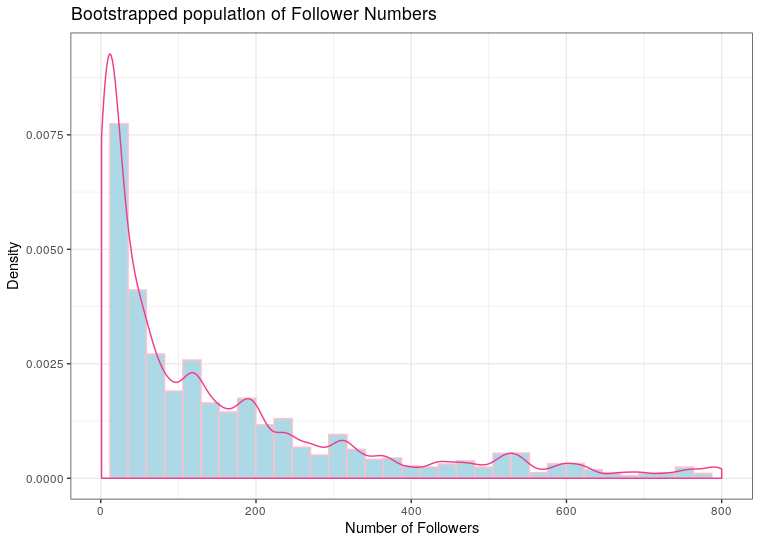
\includegraphics[width=12cm]{./Figures/BootStrap_Pop.png}
\caption{\label{fig:org2def6d4}Histogram of the bootrapped population of follower counts}
\end{figure}

\subsubsection{c.) Estimate a Confidence Interval for the population mean Follower Counts}
\label{sec:orga8a3729}
In order to perform a bootrap for the population mean value of follower counts it is necessary to:

\begin{enumerate}
\item Resample the data with replacement
\begin{itemize}
\item that is randomly select values from the sample allowing for repetition
\end{itemize}
\item Measure the statistic in concern
\item Replicate this a sufficient number of times
\begin{itemize}
\item Greater than or equal to 1000 times \cite[Ch. 5]{davison1997}
\end{itemize}
\end{enumerate}

This is equivalent to drawing a sample from a population that is infinitely large and constructed of repetitions of the sample. This can be performed in \textbf{\emph{R}} as shown in listings


\begin{listing}[htbp]
\begin{minted}[]{r}
xbar_boot_loop <- replicate(10^3, {
  s <- sample(x, replace = TRUE)
  mean(s)
  })
quantile(xbar_boot_loop, c((1-0.97)/2, (1+0.97)/2))

##       1.5%      98.5%
##   588.4189 10228.7352
\end{minted}
\caption{\label{orgf6e827d}Confidence Interval of Mean Follower Count in Population}
\end{listing}

This provides that 97\% of samples drawn from a population will contain the population mean

A 97\% probability interval is such that a sample drawn from a population will contain the population mean in that interval 97\% of the time, this means that it may be concluded with a high degree of certainty that the true population mean lies between 588 and 10228.

\begin{enumerate}
\item Alternative Approaches
\label{sec:orgbd9d114}
If this data was normally distributed it may have been appropriate to consider
bootstrapping the standard error, however it is more appropriate to use a
percentile interval for skewed data such as this, in saying that however this method is not considered to be very accurate in the literature and is often too narrow. \cite[Section 4.1]{hesterberg2015}

\begin{itemize}
\item It's worth noting that the normal \(t\) value bootstrap offers no advantage over
using a \(t\) distribution (other than being illustrative of bootstrapping
generally) \cite[Section 4.1]{hesterberg2015}
\end{itemize}


 The \texttt{boot} package is a bootstrapping library common among authors in the data science sphere
 \cite[p. 295]{james2013} \cite[p. 237]{wiley2019} that implements
 confidence intervals consistent with work by Davison and Hinkley
 \cite{ripley2020} in there texbook \emph{Bootstrap Methods and their Application}.
In this work it is provided that the \(BC_{a}\) method of constructing confidence
 intervals is  superior to mere percentile
 methods in terms of accuracy \cite[Ch. 5]{davison1997}, a sentiment echoed in the literature. \cite[Ch. 5]{carpenter2000,davison1997}

Such methods can be implemented in \textbf{\emph{R}} by passing a function to the the \texttt{boot} call as shown in listing \ref{orge00c5cb}. This provides a broader interval, providing that the true confidence interval could lie between 1079 and 16227 followers.

\begin{listing}[htbp]
\begin{minted}[]{r}
xbar_boot <- boot(data = x, statistic = mean_val, R = 10^3)
boot.ci(xbar_boot, conf = 0.97, type = "bca", index = 1)

## BOOTSTRAP CONFIDENCE INTERVAL CALCULATIONS
## Based on 1000 bootstrap replicates
##
## CALL :
## boot.ci(boot.out = xbar_boot, conf = 0.97, type = "bca", index = 1)
##
## Intervals :
## Level       BCa
## 97%   ( 1079, 16227 )
## Calculations and Intervals on Original Scale
## Warning : BCa Intervals used Extreme Quantiles
## Some BCa intervals may be unstable
## Warning message:
## In norm.inter(t, adj.alpha) : extreme order statistics used as endpoints
\end{minted}
\caption{\label{orge00c5cb}Bootstrap of population mean follower count implementing the \(BC_{a}\) method}
\end{listing}

\label{org1090609}
\bibliography{references}

\label{org4299e1e}
 \bibliographystyle{unsrt}
\end{enumerate}

\subsubsection{d.) Estimate a Confidence Interval for the population mean Friend Counts}
\label{sec:orgc66295f}
A Confidence interval for the population mean friend counts may be constructed in a like wise fashion as shown in listings \ref{org4f1a86e}. This provides that the 97\% confidence interval for the population mean friend count is between 384 and 502 (or 387 and 496 if the \(BC_{a}\) method used, they're quite close and so the more conservative percentile method will be accepted).

\begin{listing}[htbp]
\begin{minted}[]{r}
# d.) Estimate a Confidence Interval for the populattion mean Friend Count ===
# Using a Percentile Method #####################################################
ybar_boot_loop <- replicate(10^3, {
  s <- sample(y, replace = TRUE)
  mean(s)
  })
quantile(ybar_boot_loop, c(0.015, 0.985)

# Using BCA Method #############################################################
mean_val <- function(data, index) {
  X = data[index]
  return(mean(X))
}

xbar_boot <- boot(data = y, statistic = mean_val, R = 10^3)
boot.ci(xbar_boot, conf = 0.97, type = "bca", index = 1)


##     1.5%    98.5%
## 383.7619 501.5903
##
## BOOTSTRAP CONFIDENCE INTERVAL CALCULATIONS
## Based on 1000 bootstrap replicates
##
## CALL :
## boot.ci(boot.out = xbar_boot, conf = 0.97, type = "bca", index = 1)
##
## Intervals :
## Level       BCa
## 97%   (386.8, 496.7 )
## Calculations and Intervals on Original Scale
## Some BCa intervals may be unstable
\end{minted}
\caption{\label{org4f1a86e}Bootstrap of population mean follower count}
\end{listing}

\subsection{{\bfseries\sffamily FIXME} 8.1.6 Estimate a 97\% Confidence Interval for the High Friend Count Proportion}
\label{sec:orgb237d8c}
In order to bootstrap a confidence interval for the proportion of users with
above average follower counts assume that the population mean value is equal to
the sample proportion and draw a sample of the same number of observations with
that probability.

In order to bootstrap a confidence interval for the proportion of users with
above average follower counts draw samples from a population that is infinitely large copmposed of

In order to bootstrap a confidence interval for the proportion of users with
above average follower counts repeteadly draw random samples from an infinitely large population composed entirely of the sample, this can be acheived by resampling the observations of above and below as shown in listing \ref{org4f7b9f9}.

\begin{listing}[htbp]
\begin{minted}[]{r}
# 8.1.6 High Friend Count Proportion -------------------------------------------
prop <- factor(c("Below", "Above"))
## 1 is above average, 2 is below
py_hat_bt <- replicate(10^3, {
  rs      <- sample(c("Below", "Above"),
                    size = length(y),
                    prob = c(py_hat, 1-py_hat),
                    replace = TRUE)
isabove <- rs == "Above"
mean(isabove)
})
quantile(py_hat_bt, c(0.015, 0.985))


##      1.5%     98.5%
## 0.6976744 0.7601163
\end{minted}
\caption{\label{org4f7b9f9}Bootstrap of Proportion of Friends above average}
\end{listing}


Take a population of infinite size by
\end{document}
